\subsection{Dataset Selection and Characteristics}
\label{subsec:dataset}

This section outlines our dataset selection criteria and analyzes the characteristics of the chosen datasets.

\subsubsection{Dataset Selection}
In this project, we aimed to select two datasets that offer substantial variability across different aspects to evaluate the performance of Support Vector Machine (SVM) and k-Nearest Neighbors (KNN) algorithms.
The criteria for dataset selection were centered around having one dataset that is small and another that is large, allowing us to analyze both the efficiency and effectiveness of these models across differing dataset sizes.
A smaller dataset, enables rapid experimentation and comparison of SVM and KNN performance.
Meanwhile, a larger dataset, provides an excellent opportunity to evaluate the benefits of reduction methods in KNN, especially regarding storage efficiency and reduced running time.

Moreover, we wanted to assess the models' ability to handle datasets with different types of attributes.
For this purpose, we wanted to select one dataset with primarily nominal attributes and another with numerical features.
This allows us to evaluate how well each algorithm handles the representation and processing of different data types.
Additionally, class distribution was a critical factor in our selection. By choosing one dataset with a balanced distribution and another with a notable class imbalance, we aim to observe how SVM and KNN, particularly with reduction, perform in scenarios where the data is skewed.
Lastly, we prioritized finding datasets with varying levels of missing data to examine how effectively the algorithms manage incomplete information.

Based on these criteria, we selected the Hepatitis and Mushroom datasets, as they provide the most distinct and complementary combination for our evaluation.
\subsubsection{Selection Criteria}
We selected two datasets with contrasting characteristics to evaluate the performance of Support Vector Machine (SVM) and k-Nearest Neighbors (KNN) algorithms across different scenarios. Our selection criteria focused on:

\begin{itemize}
    \item Dataset size variation (small vs. large)
    \item Attribute type diversity (nominal vs. numerical)
    \item Class distribution (balanced vs. imbalanced)
    \item Missing data patterns
\end{itemize}

A smaller dataset enables rapid experimentation and initial algorithm validation, while a larger dataset allows evaluation of reduction methods' effectiveness, particularly for KNN's storage and computational requirements.

\subsubsection{Dataset Characteristics}

\begin{figure}
    \centering
    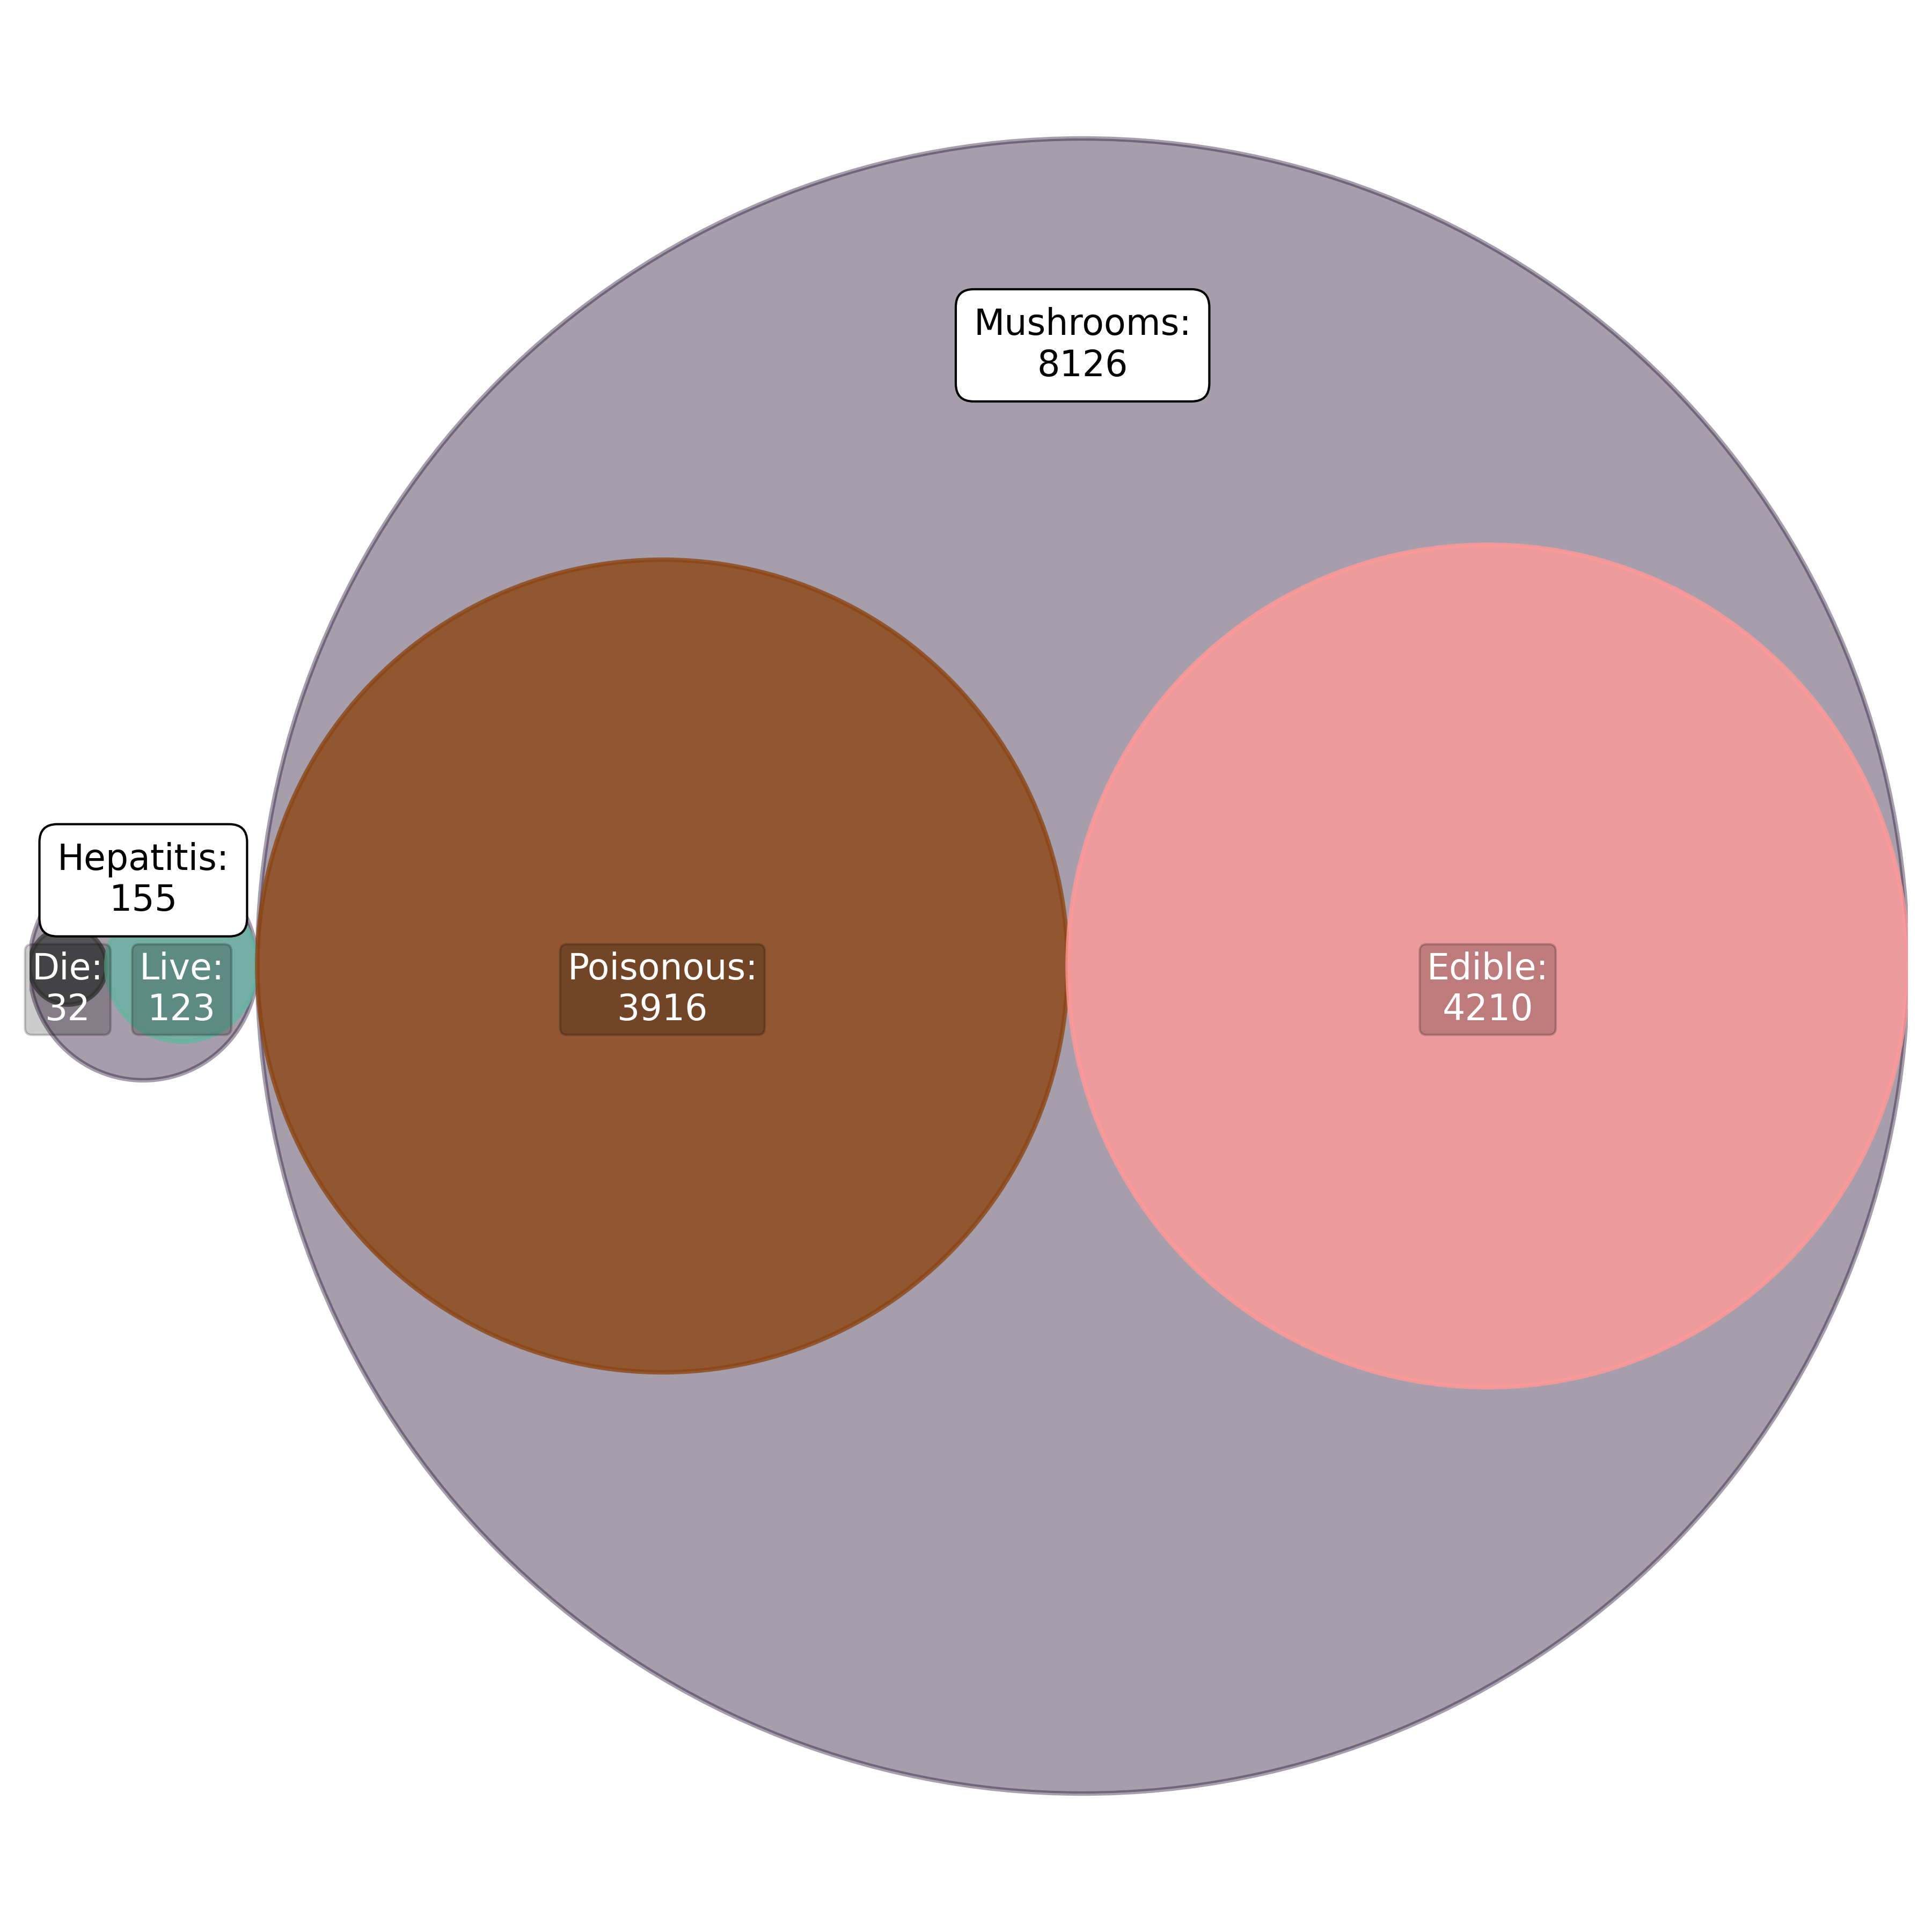
\includegraphics[width=0.5\textwidth]{figures/dataset-partitions.png}
    \caption{Size comparison of datasets used in the study}
    \label{fig:dataset-partitions}
\end{figure}

The selected datasets exhibit the following characteristics:

\begin{itemize}
    \item \textbf{Mushroom Dataset}
    \begin{itemize}
        \item 8,124 instances
        \item 22 nominal attributes
        \item Binary classification (edible vs. poisonous)
        \item Nearly balanced classes
    \end{itemize}
    
    \item \textbf{Hepatitis Dataset}
    \begin{itemize}
        \item 155 instances
        \item Mixed attribute types (both nominal and numerical)
        \item Binary classification (survive vs. die)
        \item Imbalanced classes (79.35\% majority class)
        \item 6.01\% missing values
    \end{itemize}
\end{itemize}

\begin{figure}
    \centering
    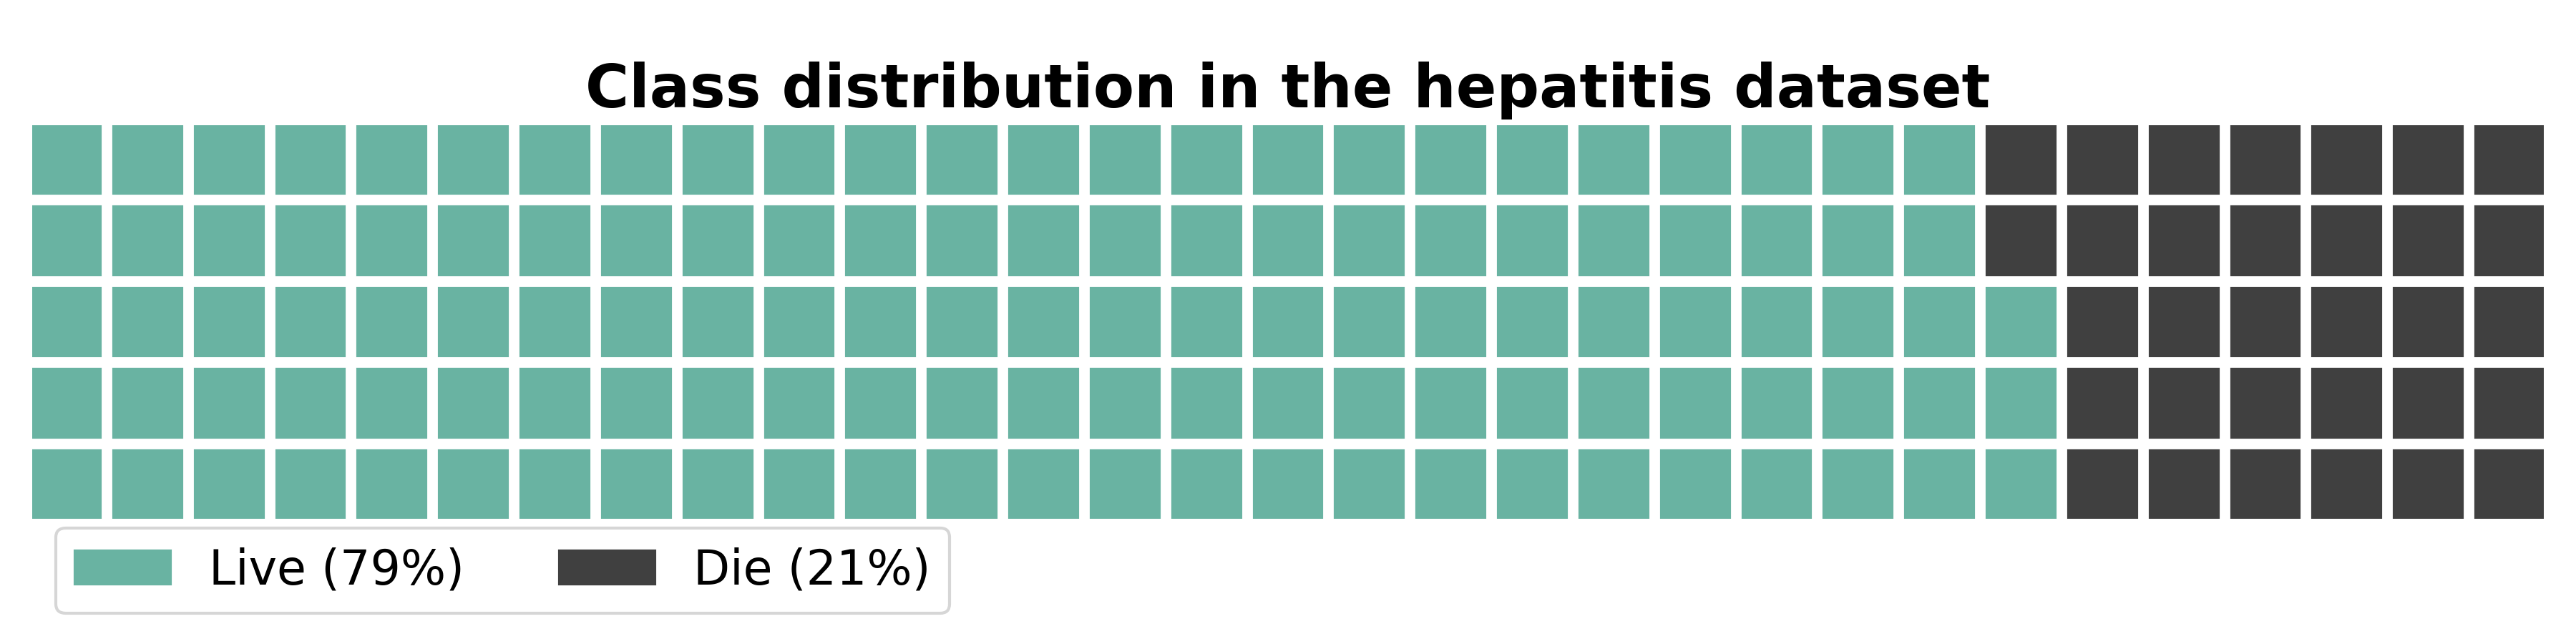
\includegraphics[width=0.45\textwidth]{figures/hepatitis-class-distribution.png}
    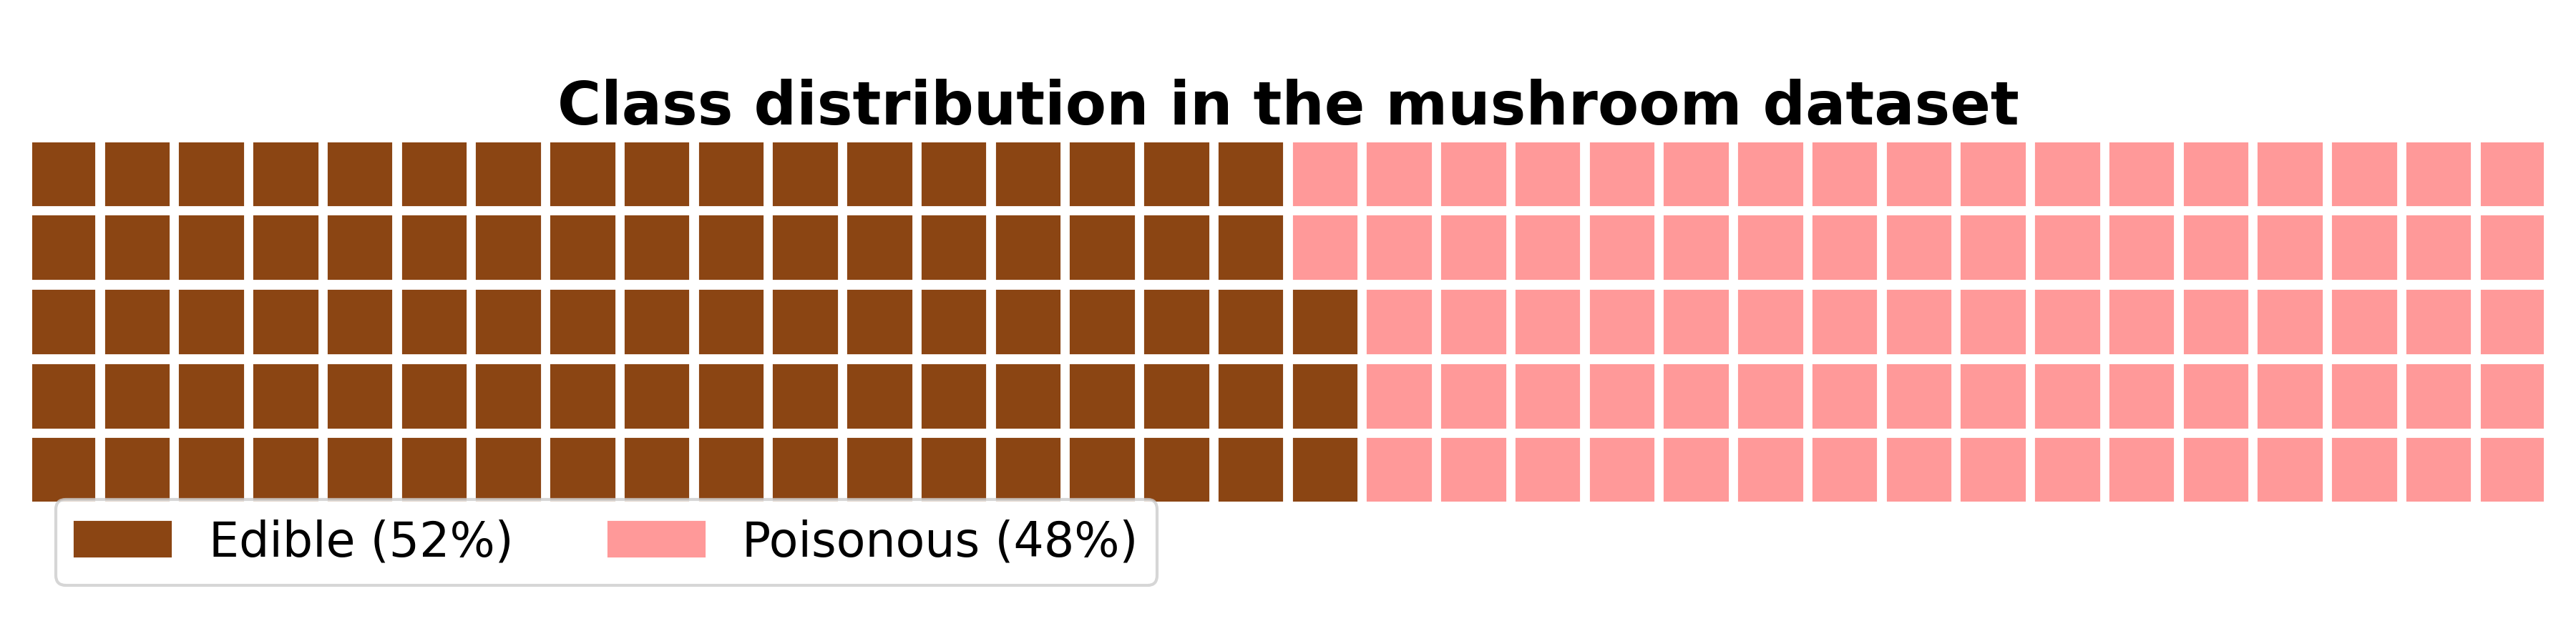
\includegraphics[width=0.45\textwidth]{figures/mushroom-class-distribution.png}
    \caption{Class distribution comparison between datasets}
    \label{fig:class-distributions}
\end{figure}

These datasets provide complementary characteristics for evaluating our algorithms' performance across different scenarios. The Mushroom dataset challenges the algorithms with its size and categorical nature, while the Hepatitis dataset tests their ability to handle mixed data types and class imbalance.